%
% Chapter 1
%
% Unifies results chapters under the framework of human genetics.

% TODO: look through dloads folder for relevant papers for each section.

\chapter{Introduction}
\label{ch:introduction}

\begin{outline}

Observable human characteristics or traits are called phenotypes.
Variation in phenotype emerges from the interplay of genetics, environment and pure chance.
The contributions of each vary from phenotype to phenotype.
Traits for which genetic variation explains a non-zero percentage of phenotypic variation are heritable.
Virtually all phenotypic traits are heritable to some degree, 
and twin studies provide upper bounds on this heritability by partitioning phenotypic variation into genetic and environmental components \autocite{polderman2015MetaanalysisHeritabilityHuman}.

Genetic variation presents a unique opportunity to probe the causal molecular mechanisms underlying phenotypes.
A mainstay of the field of human genetics is uncovering the specific genetic variants that contribute to the heritability of phenotypes through statistical association of variants and phenotypes.
Information encoded in the genome can have phenotypic consequences only after flowing through multiple molecular layers (\cref{fig:intro_sysBio}).
% NOTE: There are many mechanisms not explicitly mentioned here: PTMs, epigenetic reg, reverse transcription, RNA editing, but the predominant flow of info holds.
% Also see 
% Koonin, E.V. Does the central dogma still stand?. Biol Direct 7, 27 (2012). https://doi.org/10.1186/1745-6150-7-27
This guiding principle is the central dogma, whereby the flow is directed from DNA to RNA to protein via transcription and translation.
Barring somatic mutation, an individual's genome is fixed at conception, thus providing a causally upstream anchor that can be measured with relatively little error.
% NOTE: This was why MR was introduced in the context of family-based designs, where parent and child are of the same ancestry \autocite{daveysmith2020MendelLawsMendelian}
Although not immune to population-level confounders like stratification,
genetic association has intrinsic resistance to reverse causality, an issue that permeates observational studies on the causes of human phenotypes.

\begin{figure}
    \centering
    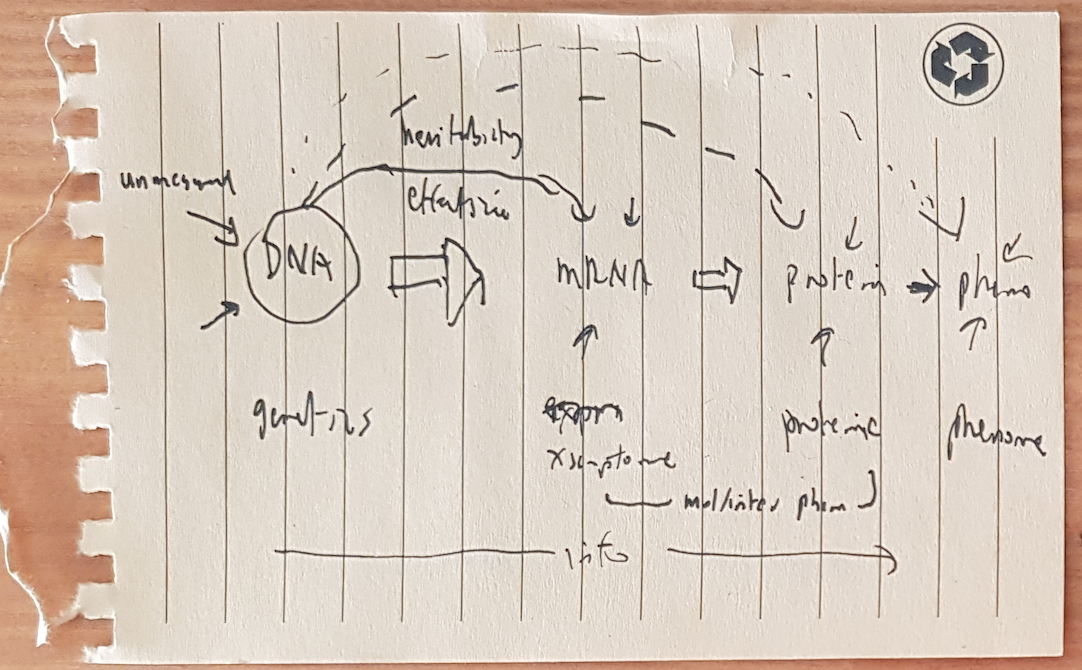
\includegraphics[width=1.0\textwidth,page=1]{mainmatter/figures/chapter_01/fig_mockup_systemsBio_Screenshot 2020-05-21 at 17.08.47.png}
    \caption{Information flow through the biological system.}
    \label{fig:intro_sysBio}
\end{figure}

\section{Genetic association studies of complex traits}
\todo{I agree the intro is built around genetics. I have tried to keep the genetics parts concise while elaborating on gene expression more in the later two sections.}

\subsection{Structure and variation of the genome}

The human genome is almost three billion \si{\bp} (base pairs) in length, 
containing \numrange{20000}{25000} protein-coding genes that span \SIrange{1}{3}{\percent} of its length, with the remaining sequence being non-coding \autocite{theencodeprojectconsortium2012IntegratedEncyclopediaDNA,1000genomesprojectconsortium2015GlobalReferenceHuman}.
% Some of the remainder is dedicated to regulatory activities \autocite{theencodeprojectconsortium2012IntegratedEncyclopediaDNA}.
Each diploid cell contains two copies of the genome, organised into 46 chromosomes comprised of 23 maternal-parental pairs: 22 pairs of homologous autosomes and one pair of sex chromosomes.
Variation in the genome between individuals in a population exists in the form of \glspl{SNP}, short indels, and structural variants.
For common population variants with \gls{MAF} \SIrange{>1}{5}{\percent},
the vast majority (\SI{>99.9}{\percent}) are \glspl{SNP} and short indels \autocite{1000genomesprojectconsortium2015GlobalReferenceHuman}.
% https://www.ncbi.nlm.nih.gov/dbvar/content/overview/
% Structural variation (SV) is generally defined as a region of DNA
% approximately 1 kb and larger in size and can include inversions and
% balanced translocations or genomic imbalances (insertions and deletions),
% commonly referred to as copy number variants (CNVs).
On average, a pair of genomes differs by one \gls{SNP} per \SIrange{1000}{2000}{\bp} \autocite{theinternationalsnpmapworkinggroup2001MapHumanGenome}.
Each version of a variant is called an allele; each individual has a maternal and parental allele at each variant.

% The Law of Dominance: An organism with alternate forms of a gene will express the form that is dominant.
% Law of Segregation: states that a diploid organism passes a randomly selected allele for a trait to its offspring, such that the offspring receives one allele from each parent.
% Law of independent assortment: states that genes do not influence each other with regard to the sorting of alleles into gametes; every possible combination of alleles for every gene is equally likely to occur.
The large number of variants in a population are inherited in a smaller number of haplotypes: 
contiguous stretches of the genome passed through generations via meiotic segregation.
The fundamental sources of genetic diversity are mutation and meiotic recombination, generating new alleles and breaking apart haplotypes into shorter ones over evolutionary time.
Variants that are physically close on a chromosome are less likely to flank a recombination event, hence more likely to cosegregate on the same haplotype (genetic linkage).
Genetic linkage is one source of \gls{LD}: the non-random association of alleles at two variants, differing from expectation based on their population frequencies and the law of independent assortment.
% LD decay takes a really long time, but there are also forces at work that generate or maintain it e.g. drift, selection, admixture, population subdivision, bottlenecks \autocite{slatkin2008LinkageDisequilibriumUnderstanding,visscher2012FiveYearsGWAS}.
\gls{LD} can be quantified by $r^2$, the squared correlation coefficient between alleles in that specific population \autocite{slatkin2008LinkageDisequilibriumUnderstanding}.

Recombination events are not distributed uniformly throughout the genome.
% TODO: Figure 3: The mosaic structure of human genetic variation. https://www.nature.com/articles/nature01400
% also see: The Structure of Haplotype Blocks in the Human Genome for original data
The genome is a mosaic of haplotype blocks delimited by recombination hotspots, 
characterised by strong \gls{LD} within blocks, and little \gls{LD} between blocks \autocite{wall2003HaplotypeBlocksLinkage,theinternationalhapmapconsortium2007SecondGenerationHuman} (\cref{fig:intro_haplotypeBlocks}).
The structure of correlated haplotypes reflects a population's unique evolutionary history, and can be used to trace the demography of populations back through time \autocite{karczewski2020AnalyticTranslationalGenetics}.

% TODO
% Figure S1. Haplotype Block Organization in Human Populations
% https://journals.plos.org/plosgenetics/article?id=10.1371/journal.pgen.0020121
% https://doi.org/10.1371/journal.pgen.0020121.sg001
% (3.6 MB TIF)
\begin{figure}
    \centering
    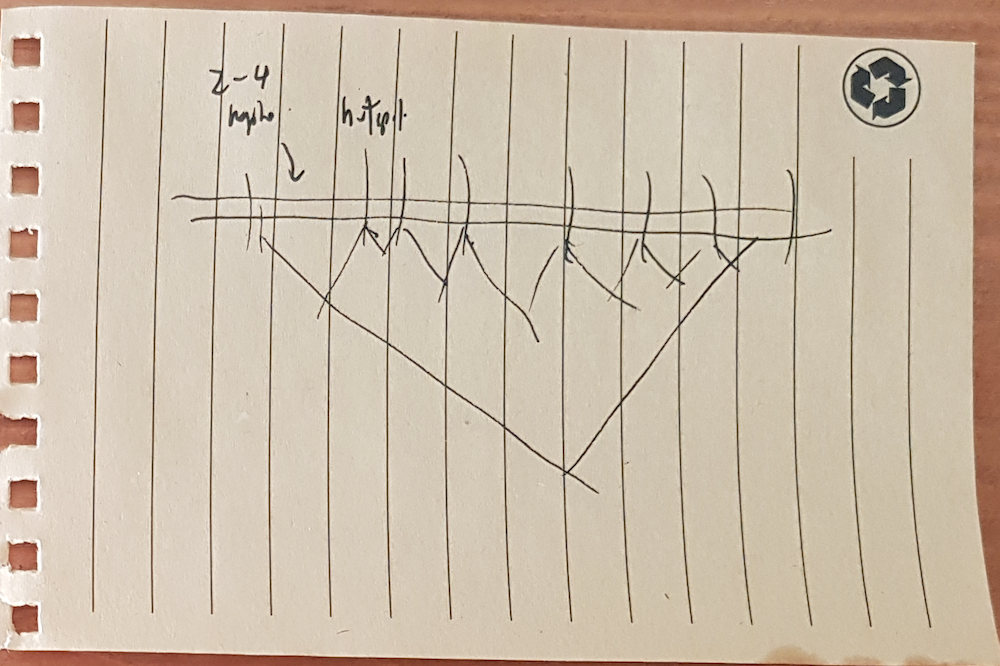
\includegraphics[width=1.0\textwidth,page=1]{mainmatter/figures/chapter_01/fig_mockup_haplotypeBlocks_Screenshot 2020-05-21 at 17.08.33.png}
    \caption{The genomic mosaic: block-like \gls{LD} structure of the genome}
    \label{fig:intro_haplotypeBlocks}
\end{figure}

\subsection{Lessons from the past fifteen years}

Genetic variants affect heritable traits by impacting the function or regulation of target genes.
How genetic variation contributes to a particular trait defines it's genetic architecture: 
the number of genes affecting that trait; and the frequencies, effect sizes, and interactions of trait-associated alleles \autocite{visscher2019Fisher1918Paper}.
The number of genes defines a spectrum of traits from monogenic (where inheritance follows simple Mendelian patterns) to polygenic (where inheritance is complex).
Proposed architectures differ greatly among complex traits, 
but all have in common that the number of genes affecting complex trait is large (ranging from dozens to many thousands),
thus the average effect size of each associated variant is small \autocite{hindorff2009PotentialEtiologicFunctional,gibson2011RareCommonVariants,boyle2017ExpandedViewComplex}.

% There are causal variants, but where are they? Two methods that exploit recombination.
% LOD score plots are very similar in concept to GWAS Manhattan plots
Since the 1980s, linkage analysis has been used to map the chromosomal position or region (loci) affecting traits by tracing the cosegregation of markers (variants with known position) with the trait in family pedigrees \autocite{altshuler2008GeneticMappingHuman,ott2011FamilybasedDesignsGenomewide,visscher2012FiveYearsGWAS}.
% \autocite{ott2011FamilybasedDesignsGenomewide}
% Linkage uses a family: since the number of recombinations per generation is small, large chunks of the genome are in linkage in a pedigree. Thus the resolution of linkage is low, but you can cover the genome with just a few hundred markers.
% Also see: https://www.genome.gov/genetics-glossary/LOD-Score for the test statistic for linkage. 
% Association uses population LD: small regions of the genome in very high LD have not been split by recombination over many generations. The resolution is higher, but you need a denser marker set.
They were complemented by early genetic association studies, which largely focused on variants in or near candidate genes selected on the basis of prior biological knowledge \autocite{hirschhorn2002ComprehensiveReviewGenetic}.
These methods saw much success for Mendelian traits, but application to most complex traits proved challenging.
Small average effect sizes meant penetrance was too low to reliably observe cosegregation problems in pedigrees \autocite{visscher2012FiveYearsGWAS}.
Early candidate gene studies were also underpowered to detect small effects \autocite{border2019NoSupportHistorical}.

The past fifteen years have seen the rise of \glspl{GWAS} that systematically test common variants selected in a comparatively hypothesis-free manner across the whole genome (\cref{fig:intro_architectureGWAS}).
Using large sample sizes to overcome small effects and large multiple testing burden, thousands of associations have been discovered for complex traits and diseases,
many robustly replicated across populations \autocite{visscher2012FiveYearsGWAS,visscher201710YearsGWAS}.
A number of take-home messages have emerged.
%
% Phenotypic variance, usually combines the genotype variance with the environmental variance. Genetic variance has three major components: the additive genetic variance, dominance variance, and epistatic variance.
% NOTE: Polygenic background modifies penetrance of monogenic variants for tier 1 genomic conditions https://www.nature.com/articles/s41467-020-17374-3
Most genetic variance is additive, the contribution of dominance and epistatic interactions is small \autocite{visscher2019Fisher1918Paper}, 
and variants with effects on multiple phenotypes (pleiotropy) are widespread \autocite{visscher2012FiveYearsGWAS}.
% It is now appreciated that complex traits have remarkable polygenicity, with many hundreds or thousands of associated loci.
Even traits that are molecular rather than whole-organism phenotypes can be remarkably polygenic, with hundreds to thousands of associated loci \autocite{sinnott-armstrong2020GWASThreeMolecular}.
\Gls{GWAS} sample sizes in the millions are increasingly commonplace,
and the discovery of new associations with ever smaller effects as sample sizes increase shows no sign of plateauing \autocite{tam2019BenefitsLimitationsGenomewide,crouch2020PolygenicInheritanceGWAS}.
% Now the biological interpretation is the greater challenge.
% TODO: add any more big take-homes from: \autocite{gallagher2018PostGWASEraAssociation,tam2019BenefitsLimitationsGenomewide}

% TODO: use PLOS https://journals.plos.org/ploscompbiol/article?id=10.1371/journal.pcbi.1002822
%
    % In general, effect size is inverse to frequency, as it is assumed there are few common variants of large effect.
%
% Genetic variants exist along a spectrum of allele frequencies and
% effect sizes. Most risk variants identified by GWAS lie within the two diagonal lines.
% Rare variants with small effect sizes are difficult to identify using GWAS, and common
% variants with large effects are unusual for common complex diseases.
% tam2019BenefitsLimitationsGenomewide
\begin{figure}
    \centering
    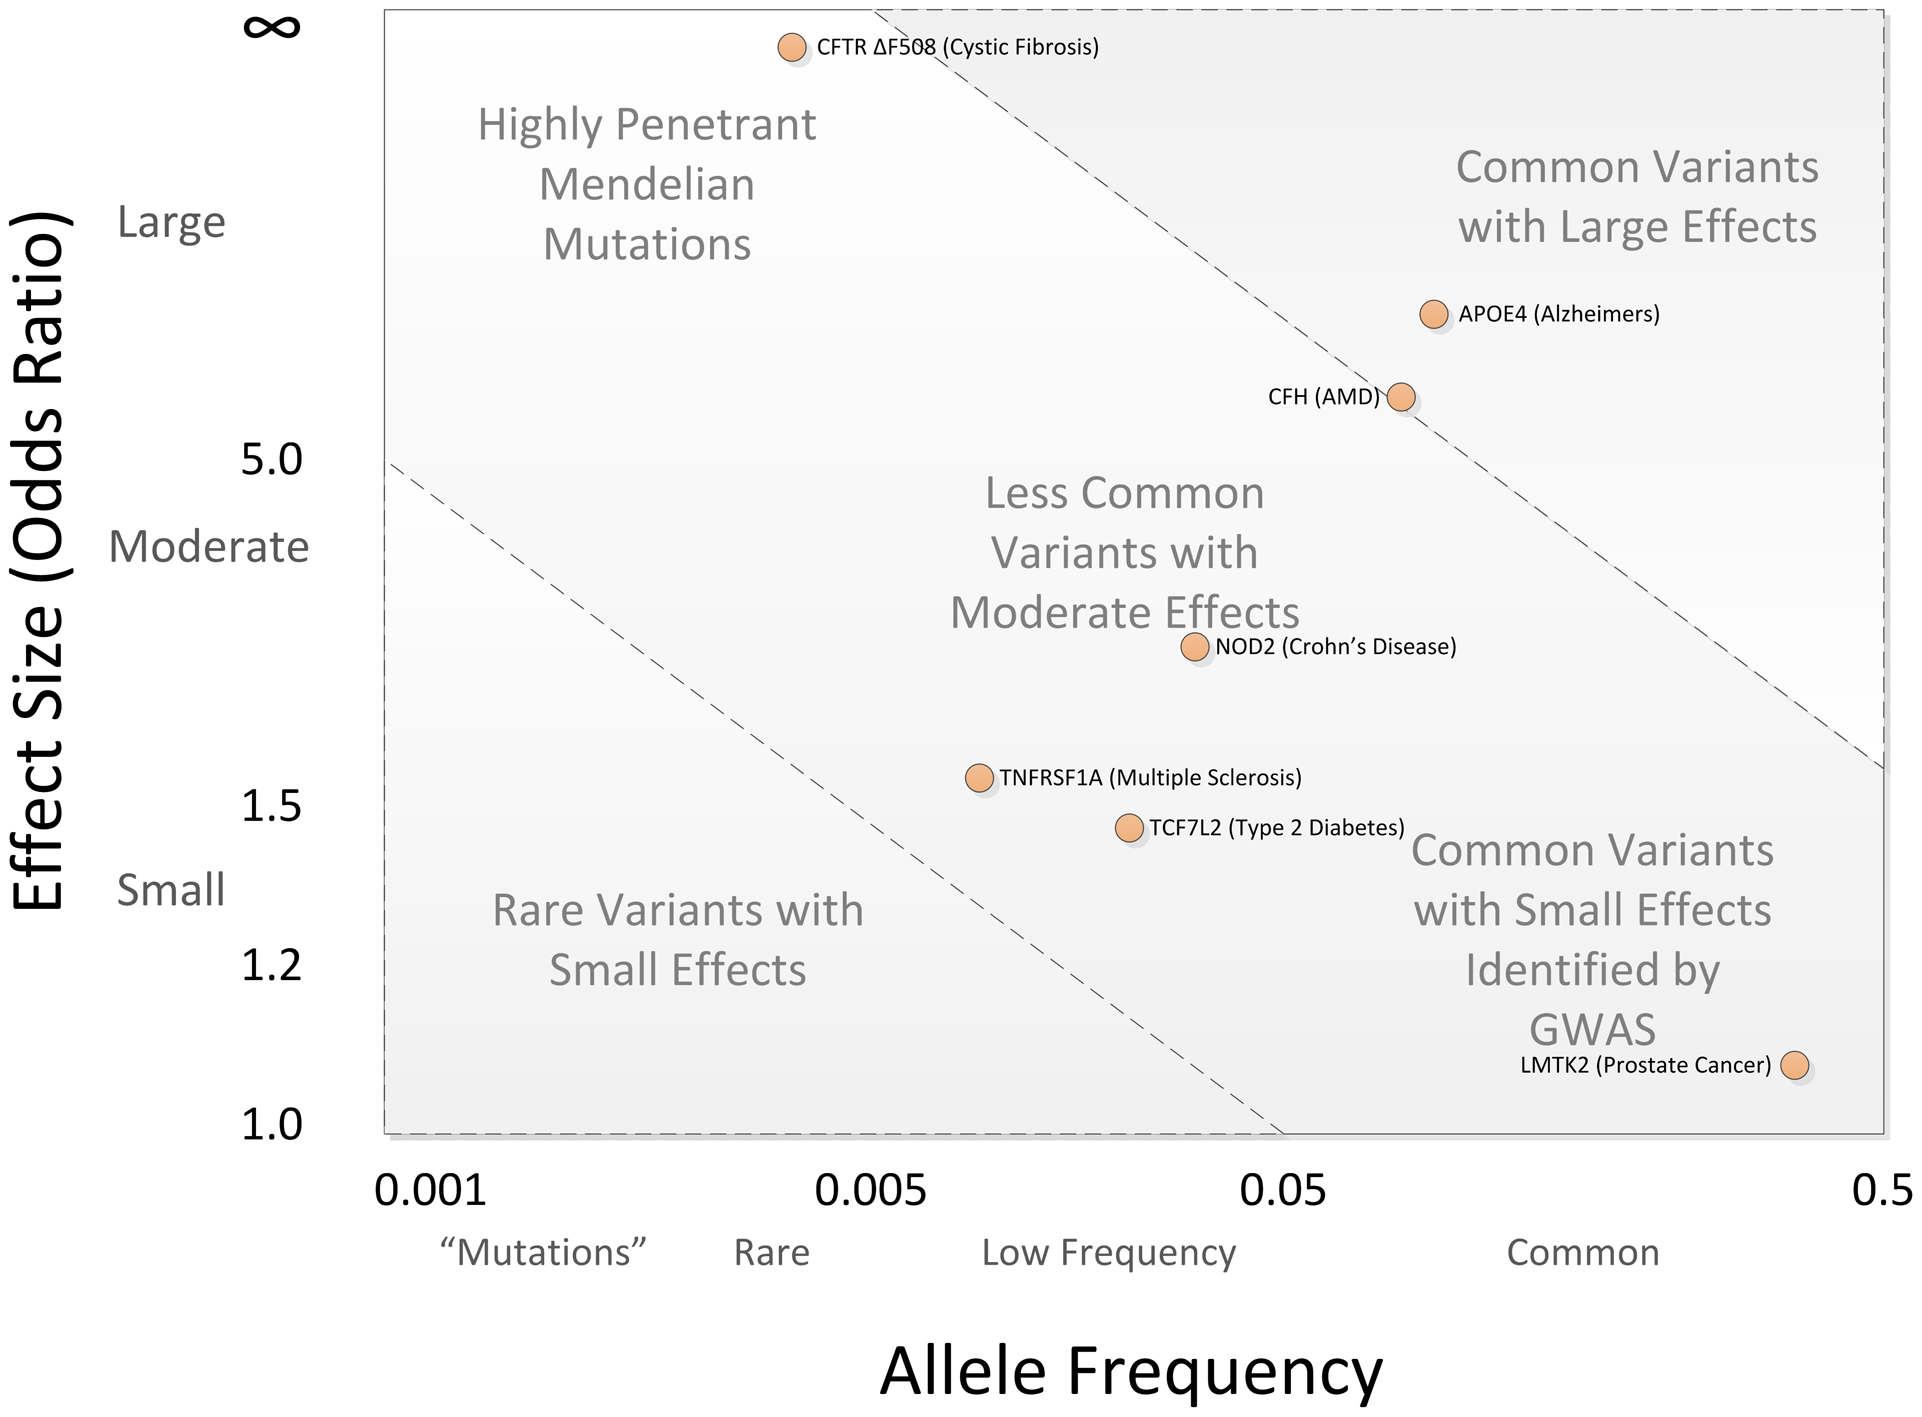
\includegraphics[width=1.0\textwidth,page=1]{mainmatter/figures/chapter_01/journal.pcbi.1002822.g001.png}
    \caption{The reach of GWAS. OR vs MAF ala tam2019BenefitsLimitationsGenomewide, extended by imputation, sample size, WGS based genotypes, but may be indistinguishable from noise at the limits}
    \label{fig:intro_architectureGWAS}
\end{figure}

\subsection{From complex trait to locus}

\glspl{GWAS} rely on the tendency of common variants on the same haplotype to be in strong \gls{LD}.
As the number of haplotypes is comparatively few, 
it is possible to select a subset of tag variants such that all other known common variants are within a certain \gls{LD} threshold of that subset. 
In practice, there is enough redundancy that the number of variants measured on a modern genotyping array (in the order of \numrange[retain-unity-mantissa=false]{1e5}{1e6}) is sufficient to tag almost all common variants  \autocite{theinternationalhapmapconsortium2005HaplotypeMapHuman,barrett2006EvaluatingCoverageGenomewide}.
Associations with unmeasured variants are indirectly detected through their strong correlation with a tag variant.
Furthermore, as unrelated individuals still share short ancestral haplotypes, 
study samples can be assigned haplotypes from a panel of haplotypes derived from reference samples by matching on the directly genotyped variants.
This process of genotype imputation allows ascertainment of many more variants not directly genotyped \autocite{das2018GenotypeImputationLarge},
but helps to recover rarer variants that are poorly-tagged \autocite{visscher201710YearsGWAS}.
Modern imputation panels enable cost-effective \glspl{GWAS} testing tens of millions of variants as rare as \SIrange{0.01}{0.1}{\percent} in diverse populations \autocite{taliun2019Sequencing53831}.

Testing large numbers of variants incurs a massive multiple testing burden, but acknowledging the correlation between variants due to \gls{LD},
there are only the equivalent of \textapprox{10^6} independent tests in the European genome, regardless of the number of tests actually performed \autocite{peer2008EstimationMultipleTesting}.
The field has thus converged on a fixed discovery threshold of $0.05 / 10^6 = \num{5e-8}$ for genome-wide significance in European populations \autocite{jannot2015108HasEmerged}, akin to controlling the type I \gls{FWER} at $\alpha = 0.05$ using the Bonferroni correction\footnote{
    The Bonferroni correction makes no assumptions about the dependence structure of the \pvalues{}, and is conservative (i.e. controls the \gls{FWER} at a stricter level than the chosen $\alpha$) even for independent tests. In fact it is always conservative unless the \pvalues{} have strong negative correlations \autocite{goeman2014MultipleHypothesisTesting}.
}.

% \subsection{Missing heritability}
%
% \1 Missing heritability refers to the observation that SNP-based heritability estimates from \gls{GWAS} fall short of additive (narrow-sense) heritability estimates from traditional quantitative methods such as twin studies.
% Perhaps unsurprisingly, it has been hypothesised that the remaining heritability lies in variants that cannot be assessed by \gls{GWAS} due to rarity or small effect.
% A classic example is the heritability of human height, estimated at 80\% by twin studies \autocite{maher2008PersonalGenomesCase},
% where considering only significant associations from \gls{GWAS} explains 5\% \autocite{maher2008PersonalGenomesCase}.
% Consideration of all common variants using mixed models (\software{GCTA}) increases the estimate to 45\% \autocite{yang2010CommonSNPsExplain},
% Recent work (\software{GREML-WGS}) suggests the full estimate of 80\% might be recoverable by also including rare and poorly tagged variants measured by \gls{WGS} \autocite{wainschtein2019RecoveryTraitHeritability}.
%
% Also see:
% 2007: Wellcome Trust Case Control Consortium landmark GWAS
% 2009: Well-known paper: Finding the missing heritability of complex diseases https://www.ncbi.nlm.nih.gov/pmc/articles/PMC2831613/
% 2018: Revisiting the Missing Heritability of Complex Diseases, Ten Years On https://www.genome.gov/event-calendar/Revisiting-Missing-Heritability-of-Complex-Diseases-Ten-Years-On
%
% NOTE: a second approach to heritability estimation is linkage disequilibrium (LD) score regression.

% \subsection{WGS/WES mitigates the coverage bias of GWAS towards known variation}
%
% \1 approx 10-fold increase in variants per tech upgrade
% \1 WES/WGS is a trade-off between sample size and genomic coverage
%     \2 Allows discovery and association with rare and novel variation, including structural variants.
%     \2 "In addition, other genome-wide scans, such as WES and WGS studies, allow testing for a burden of rare variants across shared functional units (e.g., genes) in a way that is not accessible to GWASs."
% \1 WES (covers about 40Mbp of the genome)
%     \2 covers more of the genome than GWAS
%     \2 but lower n, so lower power to do single variant associations
%     \2 needs 50x: variable coverage due to pulldown
% \1 WGS
%     \2 there is a trade-off between variant capture (n needed to observe variant) and sequencing depth (gives confidence to call variants)
%     \2 20x OK to call 90\% of singletons
%     \2 rare variants, including in nc regions
%         \3 current discovery biases, finding higher effect size vars first
%         \3 burden tests (e.g. SAIGE)
%             \4 review \url{https://www.nature.com/articles/s41576-019-0177-4}
%     \2 also gets structural variants

% \subsection{GWAS isn't designed for rare variation}
%
% There is a limit, the strategy of association is fundamentally unsuited to rare variants.
%
%     Rare Variants Association Analysis in Large-Scale Sequencing Studies at the Single Locus Level
%     https://doi.org/10.1371/journal.pcbi.1004993
%     Despite being extremely successful for common variants in GWA studies [43–46], procedures based on false-positive control are often underpowered in NGS studies involving rare variants (as illustrated in Fig 1).
%     In NGS studies with rare variants, the Signals region often degenerates due to extremely low MAF and high dimensionality.
%
% GWAS arrays also don't tag rare variants very well:
%
% https://www.ncbi.nlm.nih.gov/pmc/articles/PMC3830981/
% When the allele frequencies of two loci are very different, the r2 will never
% be very large. To see this, let's assume pA<<PB and 1-pA≈1. Then the maximum
% r2≈pA/pB*(1-pB), which is <<1 since PA is very small compared to pB. This
% indicates that causal rare variants are mostly likely to be missed in GWAS for
% single marker tests, since GWAS chips are designed to include predominantly
% common variants (e.g. MAF>0.05).
%
% Therefore, GWASs are by design powered to detect association with causal variants that are relatively common in the population.
% \autocite{visscher2012FiveYearsGWAS}

\subsection{From locus to causal variant}

By design, a significantly-associated variant from a \gls{GWAS} needs not be a variant that causally affects the trait, and may only tag a causal variant.
The resolution of the associated locus depends on the local \gls{LD} structure.
% The SNP-SNP correlation matrix
% Fine-mapping is a natural extension of mapping with higher resolution.
Fine-mapping is the process of determining which of the many correlated variants in an associated locus are most likely to be causal.
The causal variants in a locus are not necessarily the ones with the strongest associations.
State-of-the-art Bayesian fine-mapping methods take a variable selection approach, 
assigning each variant a posterior probability of causality.
A credible set of variants likely to contain all causal variants in the locus with some probability can then be determined
\autocite{schaid2018GenomewideAssociationsCandidate,wang2020SimpleNewApproach} 
The ability to separate causal and tag variants depends on factors like \gls{LD}, sample size, and the effect size and number of causal variants  \autocite{visscher201710YearsGWAS,schaid2018GenomewideAssociationsCandidate}.
It is important that the causal variant is observed, by directly genotyped or confident imputation.

% \subsection{Polygenic risk scores}
%
% Why care? PRS for prediction.
%
% First PRS
% 13. Wray, N.R., Goddard, M.E., and Visscher, P.M. (2007). Prediction of individual genetic risk to disease from genome-wide association studies. Genome Res. 17, 1520–1528.
%
% Variable prediction accuracy of polygenic scores within an ancestry group
% https://elifesciences.org/articles/48376
%
% Polygenic background modifies penetrance of monogenic variants conferring risk for coronary artery disease, breast cancer, or colorectal cancer
% https://www.medrxiv.org/content/10.1101/19013086v1

\subsection{From causal variant to target gene}

Most causal variants for Mendelian traits are coding variants (nonsense, missense, or frameshift) that impact protein sequence \autocite{chong2015GeneticBasisMendelian}.
In contrast, over \SI{90}{\percent} of \gls{GWAS} loci fall in non-coding regions \autocite{gallagher2018PostGWASEraAssociation},
and often too far from the nearest coding region to be in \gls{LD} \autocite{brodie2016HowFarSNP}.
Even if the causal variants at a \gls{GWAS} locus are fine-mapped, 
it may not be obvious how to prioritise the target genes through which those variants affect the trait.
% NOTE:
% \autocite{visscher201710YearsGWAS}:
% "For two-thirds of \gls{GWAS}-associated complex trait loci where target genes have been assigned, the implicated gene is not the nearest gene"
% but this is from SMR and TWAS studies, which may have poor performance for assigning causal genes.
A reasonable heuristic is to assign the nearest gene \gls{TSS} or body as the target, particularly for metabolite traits \autocite{stacey2019ProGeMFrameworkPrioritization}.
For improved accuracy across a variety of complex traits,
integrative methods for gene prioritisation combine variant-to-gene distance with other metrics and data types drawn from numerous external sources \autocite{stacey2019ProGeMFrameworkPrioritization,forgetta2020EffectorIndexPredict,ghoussaini2020OpenTargetsGenetics}.

% \subsection{From target gene to candidate drug}
%
% \1 gene to drug
%     \2 Are drug targets with genetic support twice as likely to be approved? Revised estimates of the impact of genetic support for drug mechanisms on the probability of drug approval
%         \3 \url{https://journals.plos.org/plosgenetics/article?id=10.1371/journal.pgen.1008489}
%     GWASing and fine-mapping complex diseases like IBD turns out a large number of common causal variants with small-effect sizes.
%     - Is polygenicity a population or individual property? i.e. are most individual IBD cases driven solely by a distribution of small-effects, or do most patients also have 1 or more large-effect rare variants that point out priority targets for their own personalised treatment?
%     - Do many of these common causal variants e.g. converge to hit on the same pathways?
%     - Otherwise, what is the use of these target discovery pipelines that output ranked lists of target genes? Could a drug designed to modulate a single protein target be expected to work for a large number of patients?
%     \2 how to drug a complex disease with no single 'candidate gene'?
%         \3 e.g. schizo is usually polygenic, future drug development could benefit from taking a multi-target approach \autocite{visscher201710YearsGWAS}
%         \3 e.g. of successful GWAS -> drug target
%             \4 drug targets with genetic support are more likely
%         \3 building allelic series

\section{Gene expression as an intermediate molecular phenotype}

\subsection{Regulation of gene expression}

% TODO: read cano-gamez2020GWASFunctionUsing

Gene regulation data are indispensable for gene prioritisation. 
Rather than directly impacting the coding sequence of a gene, 
many non-coding \gls{GWAS} loci are hypothesised to affect traits by affecting the regulation of target gene expression \autocite{gallagher2018PostGWASEraAssociation,cano-gamez2020GWASFunctionUsing}.
Unlike genotype, expression is context-dependent and dynamic across time and space.
Diverse expression programs are responsible for the myriad of cell and tissue types generated during development,
and enables adaptation in response to environmental stimuli.

Eukaryotic transcription is an intricate multi-step process involving interactions between DNA, RNA, and hundreds of proteins \autocite{cramer2019OrganizationRegulationGene}.
% RNA polymerase binds to and moves 3'->5' on the non-coding strand, creating an RNA strand that grows in a 5'->3' direction, with a sequence that corresponds to the coding strand.
Transcription of the pre-\gls{mRNA} is initiated when RNA polymerase and \glspl{TF} form part of a protein complex around the promoter region and \gls{TSS} of a gene.
\Glspl{TF} can also bind to \textit{cis}-regulatory elements such as enhancers,
which can be distant from the gene, interacting with the promoter region via DNA looping.
Transcription can only happen in regions of open chromatin, where the packing of DNA-histone complexes (nucleosomes) is loose enough that the DNA is physically-accessible to the transcriptional machinery.
Chromatin accessibility is partially determined by histone modifications such as methylation, acetylation, phosphorylation, and ubiquitination \autocite{bannister2011RegulationChromatinHistone}.
% The histone code maps modifications to activation/repression.
% The DNA itself can also be modified; methylation at CpG sites in promoters tends to repress transcription \autocite{robertson2000DNAMethylationHealth}.
The pre-\gls{mRNA} is capped at the 5' end by a modified nucleotide, and at the 3' end by a poly(A) tail.
% The 3' tail is added after cleaving the pre-mRNA off the rest of the transcribed RNA while the polymerase is still going.
% Splicing is mostly co-transcriptional.
Introns are removed, and the exons spliced together by spliceosomes that cut and rejoin the RNA at splice sites.
Different ways this occurs determines which of many alternatively-spliced transcripts is produced.
% Alternative splicing of pre-mRNA transcripts is regulated by a system of trans-acting proteins (activators and repressors) that bind to cis-acting sites or "elements" (enhancers and silencers) on the pre-mRNA transcript itself. These proteins and their respective binding elements promote or reduce the usage of a particular splice site.
Post-transcription, regulation of mature \glspl{mRNA} can occur through RNA editing and regulatory elements in 5' and 3' \glspl{UTR}.

% Functional genomics is a field of molecular biology that attempts to describe gene (and protein) functions and interactions.
% Functional genomics focuses on the dynamic aspects such as gene transcription, translation, regulation of gene expression and protein–protein interactions, as opposed to the static aspects of the genomic information such as DNA sequence or structures.
In line with the regulatory hypothesis, \gls{GWAS} variants are heavily enriched in regulatory elements annotated by functional genomics projects (e.g. ENCODE \autocite{theencodeprojectconsortium2012IntegratedEncyclopediaDNA}), including
    % In genetics, DNase I hypersensitive sites (DHSs) are regions of chromatin that are sensitive to cleavage by the DNase I enzyme. In these specific regions of the genome, chromatin has lost its condensed structure, exposing the DNA and making it accessible.
    % DNase-I hypersensitive sites sequencing (DNase-seq; [1–4]) and Assays for Transposase-Accessible Chromatin sequencing (ATAC-seq; [5, 6]) are two widely used protocols for genome-wide identification of open chromatin.
    % The overwhelming majority of disease- and trait-associated variants identified by genome-wide association studies (GWASs) lie in non-coding regions of the genome, and these variants are most strongly enriched in DHSs mapped in disease-relevant cell contexts6,7.
    regions of open chromatin, 
    % ChIP-seq combines chromatin immunoprecipitation (ChIP) with massively parallel DNA sequencing to identify the binding sites of DNA-associated proteins.
    histone binding sites, 
    \gls{TF} binding sites,
    enhancers,
    splice sites,
    and \glspl{UTR}
    \autocite{schaub2012LinkingDiseaseAssociations,maurano2012SystematicLocalizationCommon,farh2015GeneticEpigeneticFine,trynka2015DisentanglingEffectsColocalizing,nasser2020GenomewideMapsEnhancer}.
Furthermore, enrichment is often observed in particular contexts: tissues, cell types, or cell states \autocite{visscher201710YearsGWAS,gallagher2018PostGWASEraAssociation,cano-gamez2020GWASFunctionUsing}.
% NOTE: cano-gamez2020GWASFunctionUsing contains many examples of genomic feature enrichment methods, including for cell-type and stimulation specific
An example is the enrichment of fine-mapped \gls{IMID} \glspl{SNP} in CD4\textsuperscript{+} T cell enhancers, particularly to enhancers activated after stimulation \autocite{farh2015GeneticEpigeneticFine}.
% NOTE: a good example is T1D vs T2D enrichments, see cano-gamez2020GWASFunctionUsing
These results put forth expression as an important intermediate linking non-coding \gls{GWAS} variants to their associated traits, 
and help nominate trait-relevant contexts.
% NOTE: the term endophenotype has a specific definition, so here use intermediate
% Assessing the utility of intermediate phenotypes for genetic mapping of psychiatric disease https://www.ncbi.nlm.nih.gov/pmc/articles/PMC4961231/

\subsection{\Glsfmtfullpl{eQTL}}

% \1 The subset of heritable traits that are not only complex but continuous are called quantitative traits, and genetic associations for those traits are called \glspl{QTL}.
Expression in itself is a complex molecular phenotype with a heritability of \SIrange{15}{30}{\percent} \autocite{gaffney2013GlobalPropertiesFunctional}.
Genome-wide assays for expression, such as microarrays and \gls{RNAseq}, were among the earliest high-throughput technologies developed for quantifying molecular phenotypes.
Large-scale efforts such as the Genotype-Tissue Expression (GTEx) project \autocite{thegtexconsortium2020GTExConsortiumAtlas} have pioneered the study of \glspl{eQTL} other \glspl{molQTL} over the past decade \autocite{vandiedonck2017GeneticAssociationMolecular}.
% Recently more focus on other molQTLs e.g. BLUEPRINT for chromatin marks

Genetic loci associated with quantified gene expression are called \glspl{eQTL}.
Their effect sizes are large relative to variants associated with whole-organism phenotypes,
with the average \gls{eQTL} explaining \SIrange{5}{18}{\percent} of additive genetic variance for its associated gene \autocite{gaffney2013GlobalPropertiesFunctional}.
% NOTE: additive genetic variance is only part of observed variance, but a single variant explaining this much is still large. 
The \glspl{eQTL} with the largest effects tend to be concentrated near the \gls{TSS} of their target gene (\textit{cis}-\glspl{eQTL}), affecting \gls{TF} binding sites and other nearby regulatory elements.
\glspl{eQTL} further away or on a different chromosome are called \textit{trans}-\glspl{eQTL}.
The exact threshold separating \textit{cis}- from \textit{trans}- on the same chromosome is arbitrary; \SI{<1}{\mega\bp} and \SI{>5}{\mega\bp} are commonly used thresholds for \textit{cis}- and \textit{trans}-\glspl{eQTL} respectively \autocite{westra2014GenomeFunctionStudying,albert2015RoleRegulatoryVariation,vosa2018UnravelingPolygenicArchitecture}%
\footnote{
    Having a threshold is often a matter of practicality to reduce the number of variants tested.
    Assaying expression is still more costly than array genotyping, so \gls{eQTL} sample sizes are small compared to \gls{GWAS}.
    Even though \glspl{eQTL} effects are relatively large, \gls{eQTL} mapping genome-wide is still equivalent to performing \glspl{GWAS} thousands of continuous phenotypes,
    incurring enormous computational and multiple testing burdens.
    Studies focused specifically on \textit{trans}-\gls{eQTL} mapping reduce the number of tests in other ways, such as testing only trait-associated variants \autocite{vosa2018UnravelingPolygenicArchitecture}.
}.
In general, \gls{eQTL} effect size declines with distance to the \gls{TSS}, and \textit{trans}-\glspl{eQTL} have smaller effects compared to \textit{cis}-\glspl{eQTL} \autocite{vandiedonck2017GeneticAssociationMolecular}.
\textit{Trans}-\gls{eQTL} often represent \textit{cis}-\glspl{eQTL} of regulatory molecules like \glspl{TF} and RNA-binding proteins that may target many genes in \textit{trans} as master regulators \autocite{fairfax2012GeneticsGeneExpression,albert2015RoleRegulatoryVariation}.
Gathering large enough samples to detect \textit{trans}-\glspl{eQTL} remains a priority.
Most expression heritability is driven by \textit{trans}- rather than \textit{cis}- effects,
perhaps due to small but wide-reaching effects \autocite{liu2019TransEffectsGene}.
% \2 Currently discovered bulk baseline cis-eQTL have also failed to explain a lot of complex trait heritability.
%     \3 Over many complex traits, a median of 11\% heritability could be explained by mediation of GWAS loci by common (MAF > 0.01) cis-eQTL,
%     and this proportion does not include \textit{trans} or post-transcriptional effects.
%     https://www.nature.com/articles/s41588-020-0625-2
%     Averaging across traits, only 11 ± 2% of heritability was mediated by assayed gene expression levels.

\subsection{Context-dependent \glsfmtshort{eQTL}}

Like expression itself, the effects of \glspl{eQTL} are highly context-dependent \autocite{albert2015RoleRegulatoryVariation,vandiedonck2017GeneticAssociationMolecular}.
A non-exhaustive list of environmental contexts that interact with \gls{eQTL} effects includes:
    sex \autocite{yao2014SexAgeinteractingEQTLs},
    age \autocite{yao2014SexAgeinteractingEQTLs},
    ancestry \autocite{dejager2015ImmVarProjectInsights,nedelec2016GeneticAncestryNatural,quach2017LivingAdaptiveWorld},
    tissue \autocite{nica2011ArchitectureGeneRegulatory,aguet2017GeneticEffectsGene},
    purified cell type \autocite{dimas2009CommonRegulatoryVariation,dejager2015ImmVarProjectInsights,peters2016InsightGenotypePhenotypeAssociations,chen2016GeneticDriversEpigenetic,calderon2019LandscapeStimulationresponsiveChromatin},
    cell type composition in bulk samples \autocite{westra2015CellSpecificEQTL,zhernakova2017IdentificationContextdependentExpression,glastonbury2019CellTypeHeterogeneityAdipose,kim-hellmuth2020CellTypeSpecific},
    cell differentiation stage \autocite{strober2019DynamicGeneticRegulation},
    disease status \autocite{peters2016InsightGenotypePhenotypeAssociations},
    and experimental stimulation (see \cref{subsec:intro_reQTL}).
These contexts can be interdependent.
For example, tissue-dependent effects may arise from a combination of cell type-dependence and varying cell composition between tissues.

A multitude of molecular mechanisms could facilitate genotype-environment interactions at \glspl{eQTL}.
\textcite{fu2012UnravelingRegulatoryMechanisms} mapped \glspl{eQTL} in blood and four non-blood tissues (\autoref{fig:intro_reQTLmechs}), 
and proposed mechanisms that might explain discordant effects of an \gls{eQTL} allele on target gene between tissues,
assuming the \gls{eQTL} disrupts a regulatory factor's binding site.
Different effect sizes of same or opposite signs could arise 
from tissue-dependent effects of the same factor, such as activating expression in one tissue and repressing it in another e.g. due to cofactors,
or from binding of different factors in different tissues at the same site.
Tissue-specific effects could arise from tissue-specific expression of a regulatory factor.
A tissue-specific effect could also reflect tissue-specific target gene expression,
as \gls{eQTL} effect will be zero in a tissue where the target is not expressed e.g. due to chromatin inaccessibility.
Tagging of different causal variants in the two tissues, potentially with differing tagging efficiency (\gls{LD}), could generate all the above scenarios.
Furthermore, the complexity of human gene regulation means these mechanisms might be acting at epigenetic, pre-, co-, or post-transcriptional levels \glspl{eQTL} \autocite{gaffney2013GlobalPropertiesFunctional}.
Detection of context-dependent effects merely exposes differences in regulatory architecture between contexts.
Determining the underlying mechanisms may well require data types beyond just genotype and expression.

\begin{figure}
    \centering
    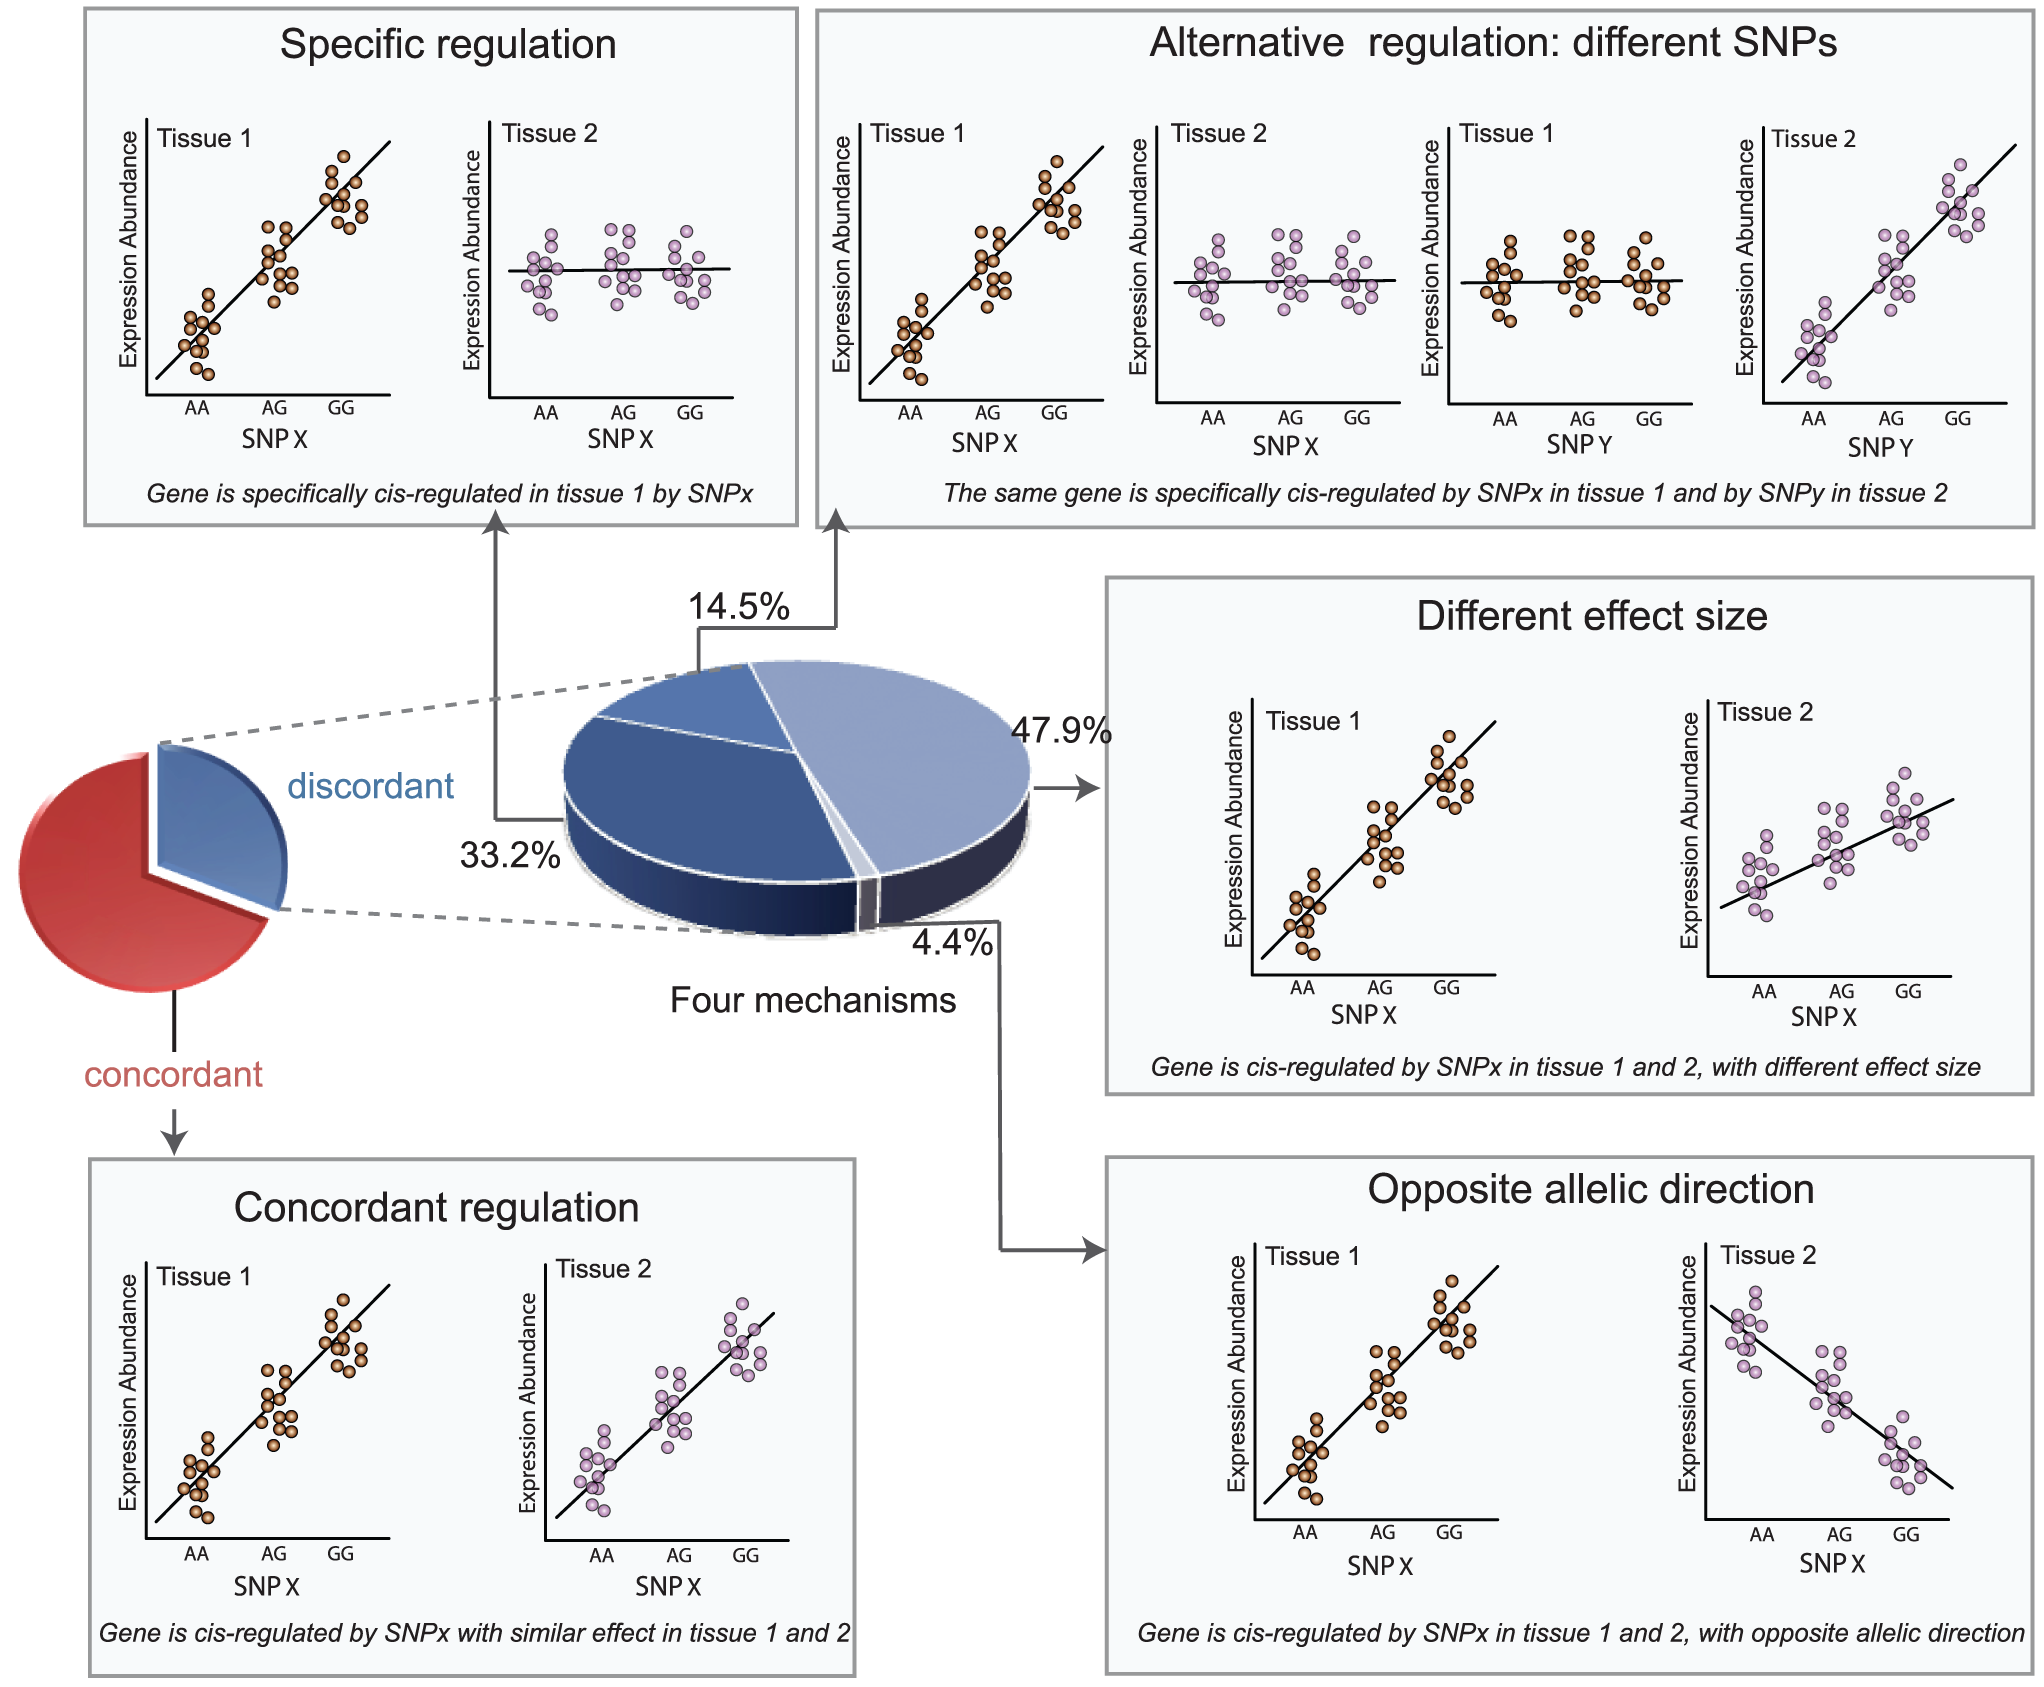
\includegraphics[width=1.0\textwidth,page=1]{mainmatter/figures/chapter_01/journal.pgen.1002431.g002.png}
    \caption{blood vs non blood. Pie charts show the proportion of different types of in pairwise comparisons of blood and four non-blood tissues.}
    \label{fig:intro_reQTLmechs}
\end{figure}

\subsection{Immune response \Glsfmtlongpl{reQTL}}
\label{subsec:intro_reQTL}

A important class of context-dependent \glspl{eQTL} are \glspl{reQTL}, 
where the interacting environment is experimental stimulation,
revealing regulatory effects not present at baseline \autocite{vandiedonck2017GeneticAssociationMolecular,huang2019GeneticsGeneExpression}.
The vast majority of \gls{reQTL} studies to date have been conducted on immune cells. 
This is not only due to the abundance of immune cells easily accessible in peripheral blood, amenable to purification and stimulation,
but because the immune system is specialised for responding to environmental perturbations in the form of infection.
Done \textit{in vitro}, variables such as cell type and abundance; and the nature, length, and intensity of stimulation can be precisely controlled.

A seminal study by \textcite{barreiro2012DecipheringGeneticArchitecture} mapped \glspl{eQTL} in monocyte-derived \glspl{DC} before and after \SI{18}{\hour} infection with \textit{Mycobacterium tuberculosis}.
\glspl{reQTL} were detected for 198 genes, 102 specific to the uninfected state, and 96 specific to the infected state. 
They observed a 1.4-fold enrichment of \glspl{reQTL} among \gls{GWAS} variants associated with susceptibility to pulmonary tuberculosis,
but no enrichment of \glspl{eQTL} shared between uninfected and infected \glspl{DC}.
From overlap of \glspl{reQTL} and \gls{GWAS} variants,
three genes were prioritised as candidates affecting tuberculosis susceptibility.
Since then, numerous \textit{in vitro} \gls{reQTL} studies have been conducted with a variety of stimulations (often cytokines, pathogens, or \glspl{PAMP}),
applied to purified \autocite{fairfax2014InnateImmuneActivity,kim2014CharacterizingGeneticBasis,hu2014RegulationGeneExpression,lee2014CommonGeneticVariants,caliskan2015HostGeneticVariation,quach2016GeneticAdaptationNeandertal,kim-hellmuth2017GeneticRegulatoryEffects,alasoo2018SharedGeneticEffects,gate2018GeneticDeterminantsCoaccessible,schmiedel2018ImpactGeneticPolymorphisms,alasoo2019GeneticEffectsPromoter,calderon2019LandscapeStimulationresponsiveChromatin,devries2020IntegratingGWASBulk,huang2020NeonatalGeneticsGene}
or mixed cell types \autocite{caliskan2015HostGeneticVariation,manry2017DecipheringGeneticControl}.

A complementary approach is \gls{reQTL} mapping with \textit{in vivo} stimulation.
An \textit{in vitro} mixture of cells cannot hope to replicate the innumerable interactions involved in human immune response.
\textit{In vivo} designs are more suitable for whole-organism stimulations and response phenotypes,
such as vaccination and vaccine-induced antibody response.

Published \textit{in vivo} \gls{reQTL} studies are comparatively few.
\textcite{idaghdour2012EvidenceAdditiveInteraction} mapped whole blood \gls{eQTL} in 94 West African children admitted to hospital for malaria, and 61 age-matched controls.
\glspl{reQTL} with a significant case-genotype interaction were detected for five genes:
\gene{PRUNE2}, \gene{SLC39A8}, \gene{C3AR1}, \gene{PADI3}, and \gene{UNC119B}.
As \gene{SLC39A8} is upregulated with T cell activation, a postulation was made that T cell activation is important to malaria infection response.
In \textcite{franco2013IntegrativeGenomicAnalysis}, whole blood \glspl{eQTL} were mapped in 247 healthy adults given \gls{TIV}.
Twenty genes involved in membrane trafficking and antigen processing were prioritised to be important to vaccine response,
having \gls{reQTL} or differential expression post-vaccination, and expression correlation with antibody response.
\textcite{lareau2016InteractionQuantitativeTrait} focused on epistatic effects of \gls{SNP}-\gls{SNP} interactions on expression fold-change after smallpox vaccination in 183 individuals.
Eleven significant interactions were found where the effect of two independent \glspl{SNP} was non-additive.
Apoptosis-related genes (e.g. \gene{TRAPPC4}, \gene{ITK}) were enriched among target genes.
Most recently, \textcite{davenport2018DiscoveringVivoCytokineeQTL}
mapped whole blood \glspl{eQTL} in 157 \gls{SLE} patients in a phase II clinical trial of an anti-IL-6 monoclonal antibody.
Nine \glspl{reQTL} where the effect was magnified in drug-exposed (drug arms) versus unexposed (placebo arm and baseline) groups
were found to disrupt the binding site of IRF4,
highlighting it as key regulatory factor downstream of IL-6.

Overall, \textit{in vivo} \gls{reQTL} studies have delivered insight into the biology of a diverse set of whole-organism phenotypes.
However, ethical requirements can limit sample size and choice of stimulation.
Many environmental factors (e.g. diet, lifestyle, immune exposures) cannot be controlled, 
potentially leading to greater experimental noise, and complicating interpretation of results.

\subsection{\Glsfmtshortpl{eQTL} for gene prioritisation}

\glspl{eQTL} are enormously valuable for target gene prioritisation after \gls{GWAS}.
They propose both target gene and mechanism of action, where the effect of variant on complex trait is mediated through expression.
\todo{Prioritisation of context is mentioned shortly.}
\Gls{GWAS} variants are indeed enriched for \glspl{eQTL} \autocite{nicolae2010TraitAssociatedSNPsAre}, but care must be taken to avoid false positives due to the abundance of \glspl{eQTL}.
At current sample sizes, \SIrange{60}{80}{\percent} of genes have at least one detectable \glspl{eQTL} \autocite{vandiedonck2017GeneticAssociationMolecular,vosa2018UnravelingPolygenicArchitecture},
and half of common variants are \textit{cis}-\glspl{eQTL} for at least one gene \autocite{liu2019AbundantAssociationsGene}.
Assuming that a locus is associated with both a trait of interest and with expression of a particular gene,
how can we separate the scenario where the same causal variants affect both trait and expression (pleiotropy),
from coincidental overlap between distinct sets of causal variants that may possibly in \gls{LD}?
Bayesian colocalisation methods address this by extending fine-mapping to multiple phenotypes \autocite{burgess2018InferringCausalRelationships,wallace2020ElicitingPriorsRelaxing,hukku2020ProbabilisticColocalizationGenetic}.
Using information from all variants in the locus, 
they estimate the posterior probability that the same causal variants are associated with both phenotypes,
distinguishing pleiotropy from \gls{LD}.

Given the effect of an \gls{eQTL} can be starkly context-dependent, 
\gls{eQTL} datasets from trait-relevant contexts are most useful for gene prioritisation.
For instance, immune \textit{in vitro} \gls{reQTL} are enriched more so than non-\gls{reQTL} among \gls{GWAS} associations for immune-related phenotypes such as
susceptibility to infectious \autocite{barreiro2012DecipheringGeneticArchitecture,manry2017DecipheringGeneticControl}
and immune-mediated diseases \autocite{manry2017DecipheringGeneticControl,kim-hellmuth2017GeneticRegulatoryEffects}.
Knowledge of cell type-specific as well as shared \gls{eQTL} effects 
finds many additional colocalisations with complex traits \autocite{kundu2020GeneticAssociationsRegulatory,kim-hellmuth2020CellTypeSpecific}.
The increasing number of context-dependent datasets available for large-scale colocalisation analyses means \glspl{eQTL} can propose not just target gene and mechanism, but also the specific environments most relevant to a trait.

% coloc then finemap
% coloc can also can help fine mapping, as large effect = smaller n required = able to do denser genotype by e.g. wgs, so smaller credible sets at much lower sample sizes
% "Overall, our findings suggest that fine-mapping applied to disease-colocalising regulatory QTLs can enhance the discovery of putative causal disease variants and provide insights into the underlying causal genes and molecular mechanisms."
% https://www.biorxiv.org/content/10.1101/2020.01.15.907436v1

\section{Phenotypes of immune response}

\subsection{An overview of the immune system}

\1 essential for defense, but dysregulated
    % TODO: janeway ch1 and 2
    \2 The immune system consists of complex interaction of many cell types
    \2 two lineages, lymphoid and myeloid linages
    \2 two major arms, innate and adaptive.
    \todo{specifically introduce cell types mentioned in later chapters}
        \3 pbmcs
        \3 MHC
        \3 humoral and celluar response
    \2 complex interactions through cell surface receptors and signalling molecules

\subsection{High-throughput immunology}

% TODO: read davis 2018 and 2020
\1 systems immunology systems rather than reductionist approach to study a intricate system
\1 omics studies of interactions with and between all these layers of the immune system come under the broad umbrella of systems immunology
% TODO: longitudinal: rules out reverse causal by establishing temporal
    \2 Longitudinal designs and high-throughput technologies to quantify the components of the immune system at baseline, and in response to perturbations.
        \3 genomics, epigenomics, transciptomics, proteomics, cell counts
    \2 Whatever the perturbation, just like for most phenotypes, immune response varies between individuals
    \2 Main types of study are descriptive:
        \3 finding correlations between the components of the immune system, and with phenotypic response
    \2 predictive:
        \3 Use assayed information to predict phenotypic response from molecular assays
    \2 causal:
        \3 Mechanisms of response are important to understand e.g. 
            \4 what mechanisms promote effective responses to pathogens and vaccines
            \4 impede dysregulated responses that lead to immune-mediated disease such as IBD.
    \2 Natural genetic variation can be leveraged, representing small scale perturbations that are causally anchored \autocite{tsang2015UtilizingPopulationVariation,villani2018SystemsImmunologyLearning}
    % TODO: Writ large
        \3 Overall estimates of the heritability of many immune parameters, such as cell composition and serum protein levels, lies between 20-40\% \autocite{liston2016ShapingVariationHuman,brodin2017HumanImmuneSystem,patin2018NaturalVariationParameters,liston2018OriginsDiversityHuman}
        \3 Genetic regulation is more important for the innate immune system than the adaptive immune system \autocite{patin2018NaturalVariationParameters}.

% \subsection{Genetic effects on the healthy immune system}
%
% \1 Heritability of immune phenotypes is not only restricted to the expression phenotypes discussed above.
%     \2 Systems studies of interindividual variation in the healthy immune system shows many aspects of the immune system are heritable and complex.
%         \3 <Systems immunology: just getting started \url{https://www.nature.com/articles/ni.3768}>
%     \2 Immune parameters are influenced by age, sex, seasonality, and chronic infection \autocite{brodin2015VariationHumanImmune,liston2016ShapingVariationHuman,brodin2017HumanImmuneSystem,patin2018NaturalVariationParameters,liston2018OriginsDiversityHuman} \url{https://www.nature.com/articles/ncomms8000},
    % TODO: define aspects, parameters
    % TODO: add https://www.nature.com/articles/ni.3371 "The cellular composition of the human immune system is shaped by age and cohabitation"
%     but most individuals have a healthy baseline immune state that is individual-specific,
%     and relatively stable over time \autocite{liston2016ShapingVariationHuman,brodin2017HumanImmuneSystem,lakshmikanth2020HumanImmuneSystem}.
    % TODO: stable, yet varies by age? respecify scale of stability
    % TODO: add https://www.sciencedirect.com/science/article/abs/pii/S0952791520300698 "Understanding immune variation for improved translational medicine"
%     \2 Overall estimates of the heritability of many immune parameters, such as cell composition and serum protein levels, lies between 20-40\% \autocite{liston2016ShapingVariationHuman,brodin2017HumanImmuneSystem,patin2018NaturalVariationParameters,liston2018OriginsDiversityHuman}
%     \2 Genetic regulation is more important for the innate immune system than the adaptive immune system \autocite{patin2018NaturalVariationParameters}.
%
% \1 given genetic control of healthy system, perhaps not surprising that immune response to perturbation traits are also complex
%     \2 also, as discussed in the context section above, context-dependent genetic effects may not be apparent in the baseline healthy state, stimulation is required
%     \2 since a central goal of systems immunology is to establish causal relationships between the many components of the immune system
%         \3 Natural genetic variation can be leveraged, representing small scale perturbations that are causally anchored \autocite{tsang2015UtilizingPopulationVariation,villani2018SystemsImmunologyLearning}
%     \2 In this context, immune in vivo reQTL studies can be considered as controllable perturbation studies of the activated immune system
%         \3 Studies of natural infection are complicated by e.g. determining exposure, ethics, dose
%     \2 Simultaneously provides insight in to the biology behind those specific responses
%     \2 Two immune perturbations considered in this thesis are vaccines and biologic drugs.

        % TODO:
% \subsection{Leveraging perturbations}
        % natural and experiemtnal

\subsection{Immune response to vaccination}
% NOTE: technically vaccines are biologics
\todo{this is a general systems vaccinology review. specific flu studies are reviewed in ch2}

\1 One of the earliest applications of systems immunology was to vaccine response, leading to the sub-discipline of systems vaccinology.
    % TODO: basic principles here, then deep dive into specifics of the Pandemrix vaccine type
    \2 <general summary of biology of vaccine response, specific flu vaccine biology goes in ch2>
        \3 Vaccines stimulate the immune system with pathogen-derived antigens to induce effector responses (primarily antigen-specific antibodies) and immunological memory against the pathogen itself.
        \3 These effector responses are then be rapidly reactivated in cases of future exposure to the pathogen, mediating long-term protection.
        \3 Non-Ab mediated responses [...]
        % \3 <a bit more on innate/adaptive distinction, B/T lineage distinction>
    \2 Vaccination has enormous impact on global health \autocite{greenwood2014ContributionVaccinationGlobal}
    \2 But traditional vaccine dev is empirical (classical "isolate, inactivate, inject" paradigm), often successful vaccine dev does not offer insights into the mechanisms of efficacy 
    \2 The immunological mechanisms that underpin a specific vaccine's success or failure in a given individual are often poorly understood.
    % <For the majority of licensed vaccines, there is a lack of understanding regarding the molecular mechanisms that underpin this variation in host immune response.>
    \2 A vaccine that is highly efficacious in one human population may have significantly lower efficacy in other populations.
    Particularly challenging populations for vaccination include the infants and elderly, pregnant, immuno compromised patients, ethnically-diverse populations, and developing countries.
        \3 e.g. variable vaccine efficacy of rotavirus vaccine
        \3 e.g. variable efficacy of flu vaccine \url{https://www.sciencedirect.com/science/article/pii/S1473309918304900}

% TODO: figure on innate phase then adaptive response to vacc

% TODO: first year report for sysvacc intro
\1 Systems vaccinology is the application of -omics technologies to provide a systems-level characterisation of the human immune system after vaccine-perturbation.
    % \2 These systems vaccinology studies often consider longitudinal measurements of the transcriptomic, cellular, cytokine, and antibody immune responses following vaccination.
    % \2 Measurements are taken at multiple molecular levels (e.g. genome, transcriptome, proteome), and molecular signatures that correlate with and predict vaccine-induced immunity are identified.
    \2 Systems vaccinology has been successfully applied to a variety of licensed vaccines [yellow fever, influenza ...], and also to vaccine candidates against [HIV, malaria ...], resulting in the identification of early transcriptomic signatures that predict vaccine-induced antibody responses.
    \todo{define what a signature is in terms of correlation and prediction}
        \3 <add more references to lists [...] of what vaccines have been studied>
        % TODO use sysvacc\_review\_docx
    \2 Has revealed many influences on vaccine response (age, sex, dose, adjuvants, expression signatures, microbiome, strain etc.)
    \2 So far, studies have been mainly descriptive and predictive.
    \2 Identifying causal relationships can inform more mechanism-based and cost-effective design (rational paradigm), and the move towards personalised vaccinology.
    \2 Studies of impact of host genetics on response are underrepresented \autocite{linnik2016ImpactHostGenetic}

\1 Like for other complex traits, from twin studies it's known that vaccine Ab responses are heritable.
    \2 Moving out of the candidate gene era (e.g. \url{https://www.ncbi.nlm.nih.gov/pmc/articles/PMC3570049/}) into GWAS.
    % TODO: are there mendellian associations?
    \2 Heritability of vaccine response phenotypes \autocite{oconnor2013CharacterizingVaccineResponses}
    \2 Many loci have been implicated by GWAS e.g. HLA \autocite{oconnor2013CharacterizingVaccineResponses,mooney2013SystemsImmunogeneticsVaccines,mentzer2015SearchingHumanGenetic,linnik2016ImpactHostGenetic,scepanovic2018HumanGeneticVariants,dhakal2019HostFactorsImpact}
    % TODO: add brodin twin study
    \todo{find best GWAS ref, probably mooney2013SystemsImmunogeneticsVaccines, then prune and reassign these citations}
    % \2 Also, phenotypes such as adverse events have been studied e.g. \url{https://pubmed.ncbi.nlm.nih.gov/25344690/}
    \2 Overall, systems vacc studies that include genetics (sometimes dubbed as vaccinogenomics studies) are nowhere near as mature compared to the trait to gene pipeline described in above e.g. applied to complex disease

\subsection{Immune response to anti-TNF biologics}
\todo{cut this section (???)}
<Considering whether I need a section here on anti-TNFs analogous to the above systems vaccinology section. Much anti-TNF response literature is already reviewed in chapter 4 introduction though, so maybe no point duplicating.>
%
%
% TODO: merge this into intro ch4
% \1 <quick anti-tnf summary, specific ADA/IFX biology goes in ch4>
%     \2 biologics are drugs synthesised using a living organism, typically proteins
%     \2 cause immune response due to having immune targets, or immunogenecity because or their large and complex structure vs chem synth small molecule drugs
%     \2 one of the largest classes are anti-TNFs
%     \2 anti-TNFs (or TNF inhibitors), are drugs that suppress the activity of the TNF signalling pathway of the immune system
        % \3 TNF is an inflammatory cytokine ... inflammation is ...
%     \2 they are used to treat immune-mediated inflammatory diseases e.g. rheumatoid arthritis, Crohn's disease, psoriasis and ankylosing spondylitis.
    % Currently, five biologic agents targeting TNF are approved for the treatment of rheumatoid arthritis (RA), inflammatory bowel disease (IBD; for example, Crohn disease and ulcerative colitis), psoriasis, psoriatic arthritis, ankylosing spondylitis, juvenile idiopathic arthritis (JIA) and, most recently, hidradenitis suppurativa4,5 (TABLE 1).
%         \3 indicated for many IMIDs e.g. rheumatoid arthritis, Psoriasis, ankylosing spondylitis. \autocite{lichtenstein2013ComprehensiveReviewAntitumor,kalliolias2016TNFBiologyPathogenic,mulhearn2019UsingImmunophenotypePredict}
%     \2 an enormous amount of money is spent on them: anti-TNF biologics are some of the largest market share pharmaceuticals
%     \2 some proportion of patients fail. given the expenditures, it would be good to predict this
%
% TODO: figure on TNF pathway with drug targets
% TODO: table of biologics with costs
%
% TODO: merge this intro discussion ch4
% \1 <expression signatures of response to anti-TNFs>
%     \2 Systems immunology has also been applied to anti-TNFs
%     \2 have been detected e.g. for RA <"Validation study of existing gene expression signatures for anti-TNF treatment in patients with rheumatoid arthritis" \url{https://pubmed.ncbi.nlm.nih.gov/22457743/}>
    % e.g. https://www.ncbi.nlm.nih.gov/pmc/articles/PMC6614444/
%     \2 most detected in small cohorts, many require validation
%
% TODO: merge this intro discussion ch4
% \1 <genetics of anti-TNF response>
%     \2 pharmacogenomics is the study of the role of genetics in beneficial and adverse effects of drugs and theraputics \url{https://doi.org/10.1016/S0140-6736(19)31276-0}
%     \2 some implementation in clinic already e.g. screening for certain allele-drug combos \url{https://www.nature.com/articles/nature15817} \url{https://academic.oup.com/bmb/article/124/1/65/4430783}
%     \2 GWAS in the pharmacogenomics field \url{https://www.ncbi.nlm.nih.gov/pmc/articles/PMC3003940/} \url{https://www.futuremedicine.com/doi/full/10.2217/pgs-2018-0204}
    % Genome-wide association studies (GWAS) have proven to be a more successful approach for this objective. To date, eight GWAS on anti-TNF response in RA have been performed (22–29), identifying several loci associated at a genome-wide scale. From these, variation at MED15, GFRA1, PDE3A-SLCO1C1, and CD84 has been replicated in, at least, an independent cohort of patients (30).
%     \2 GWAS studies of anti-TNF response in RA \url{https://www.ncbi.nlm.nih.gov/pmc/articles/PMC6614444/}
        % \3 also add Discovery studies from \url{https://www.ebi.ac.uk/gwas/efotraits/EFO_0004653}
    % \2 TODO: \url{https://www.ebi.ac.uk/gwas/search?query=TNF},
    % also google anti tnf immune response gwas
        % e.g.
        % https://www.ncbi.nlm.nih.gov/pmc/articles/PMC6150911/
        % https://journals.plos.org/plosone/article?id=10.1371/journal.pone.0213073
%         \3 a few validation studies attempted e.g. \url{https://www.ncbi.nlm.nih.gov/pmc/articles/PMC5937760/}
%
% \1 a lot of studies also done for CD and IBD (described in ch4)

\section{Thesis overview}

\1 My thesis focuses on two specific instances of in vivo immune response: antibody response to pandemic influenza vaccine in healthy individuals, and clinical response to biologic anti-TNF therapy for CD patients.
\1 <By chapter context-content-conclusion overview.>
    \2 <ch 2: systems vaccinology study of Pandemrix>
        \3 context: existing Sobolev study of expression differences between pandemic flu vaccine R/NR had small sample size and binary phenotype
        \3 content: meta-analysis of existing array with new RNAseq data and continuous phenotype
        \3 conclusion: distinct innate and adaptive expression response at d1 and d7; heterogeneity between array and RNAseq. significant expression differences between R/NR in meta-analysis at the gene set level
    \2 <ch 3: in vivo reQTL study of Pandemrix>
        \3 context: relatively few studies have assessed the impact of genetic variation on expression response to flu vaccine
        \3 content: reQTL analysis for flu vaccine at d0, d1, d7. many reQTLs including sign flips. no particular gene set enrichments. evidence of cell type interactions at top hits.
        \3 conclusion: difficult to separate out modifying effect of cell composition. this may be a fundamental flaw in the study design
    \2 <ch 4: systems immunology and reQTL study of response to anti-TNF treatment in CD>
        \3 context: studies on expression signatures of anti-TNF PNR have been small
        \3 content: R/NR comparison with larger n, at baseline, w14, and over time. reQTL analysis over 4 timepoints. 
        \3 conclusion: a few hits for PNR at baseline. much stronger expression differences stronger at w14, then maintained until w54. Weak evidence for reQTLs, probably due to smaller magnitude of cell proportion changes over time vs the previous chapter.
    \2 <discussion: limitations, future outlook>
        \3 main themes and parallels tying together the thesis
        \3 shared set of limitations permeating all chapters
        \3 recommendations for future analyses and study design
        \3 future outlook for the fields of systems studies of immune response% vaccinogenomics and pharmacogenomics

\end{outline}
